% 第 18 节：强子谱的格点计算
% R. Gupta, "Introduction to Lattice QCD" (arXiv:hep-lat/9807028)

\chapter{强子谱的格点计算}

成功的谱计算将检验QCD。格点分析的基本步骤已在第~4 节和第~17 节中讨论。对于给定的一组输入参数，某个给定态的质量由连通两点关联函数的指数衰减速率确定
\begin{equation}
\Gamma(\tau) \equiv \langle O_f(\tau) O_i(0) \rangle - \langle O_f \rangle \langle O_i \rangle
= \sum_n \frac{\langle 0 | O_f | n \rangle \langle n | O_i | 0 \rangle}{2 M_n}\, e^{-M_n \tau}.
\label{eq:2pt}
\end{equation}

我们将假设，对 $n$ 的求和被限制到所需态上，做法是：(i) 优化 $O_i$ 和 $O_f$，使其与波函数有大的重叠，即让所需态 $\langle n | O | 0 \rangle$ 大而其余的小；(ii) 增加统计量，使信号延伸到足够大的 $\tau$，此时来自更高态的剩余污染均可忽略；(3) 对 $O_i$ 或 $O_f$ 之一作零动量投影。我还将进一步假设，可能态的谱是离散的，并且存在质量间隙。于是，为了提取 $M$，定义一个有效质量是有用的
\begin{equation}
M_{eff}(\tau) = \log\!\left( \frac{\Gamma(\tau-1)}{\Gamma(\tau)} \right)
\label{eq:meff}
\end{equation}
它在极限 $\tau \to \infty$ 下收敛到所需的值。$M_{eff}(\tau)$ 行为的两类不同态（$\pi$介子与核子）以及 $O_i$、$O_f$ 两类不同选取的剖析如图~\ref{fig:22} 和图~\ref{fig:23} 所示。值得注意的要点是：
\begin{itemize}
\item 对渐近值 $M$ 的收敛既可以从上也可以从下，取决于 $O$ 的选取。只有当 $O_f = O_i^\dagger$ 时，关联函数才正定，收敛才是单调的且自上而下。
\item 对于 $O_f \neq O_i^\dagger$，收敛依赖于各态贡献之间的精细相消。相对符号由两个振幅的乘积 $\langle n | O_f | 0 \rangle \langle n | O_i | 0 \rangle$ 给出。由于态 $|n\rangle$ 的这个符号可正可负，收敛既不保证是单调的，也不保证自上而下。
\end{itemize}

\begin{figure}[htbp]
\centering
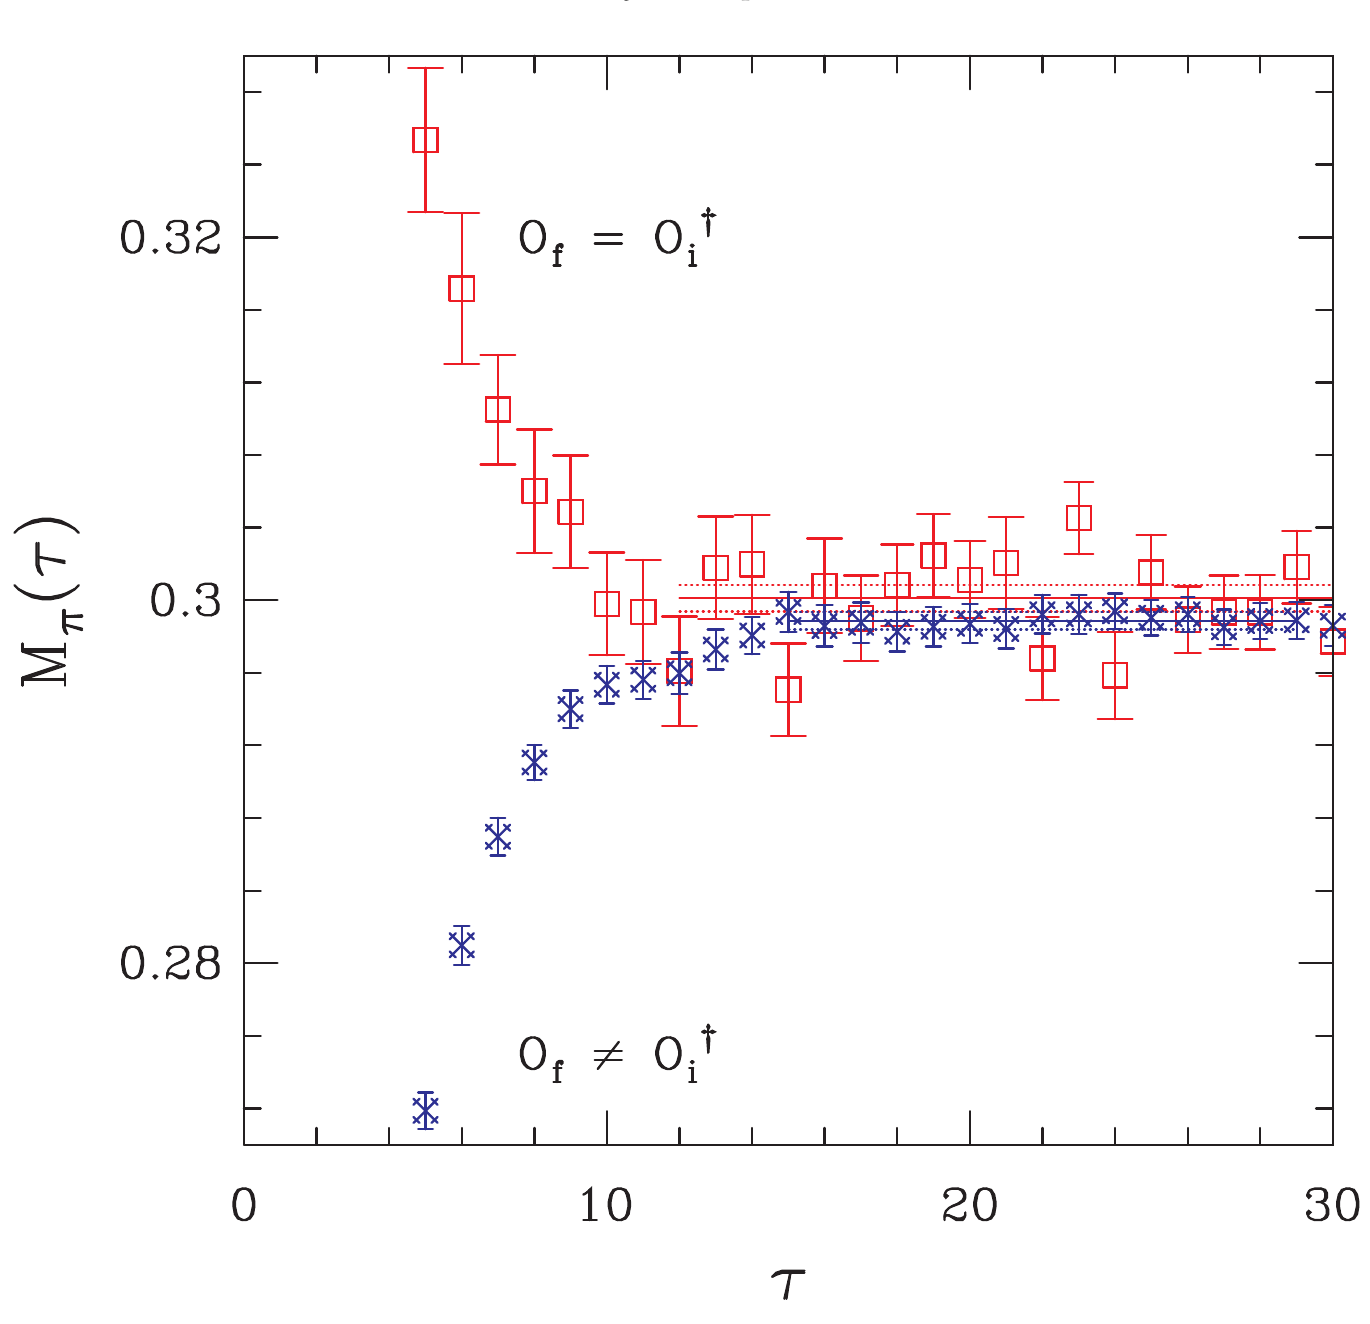
\includegraphics[width=0.8\textwidth]{images/fig22.png}
\caption{$M_\pi$ 随 $\tau$ 变化的有效质量图。水平线表示 $M$ 渐近值的估计以及拟合中所用平台区的范围，点线则显示误差。方块表示涂抹–涂抹插值算符（$O_f = O_i^\dagger$）的数据，异形叉号表示采用墙定域算符的数据。}
\label{fig:22}
\end{figure}

\begin{itemize}
\item 激发态的贡献在小 $\tau$ 处最为明显，此时 $M_{eff}$ 在变平之前迅速变化。对于处于这一平坦（称为平台）区域的 $\tau$，可以假设在数值精度内只有最低态的贡献是显著的。
\item 平台区开始的位置（在 $\tau$ 上）及其长度依赖于插值算符。
\item 对于有限的统计样本，平台区并非平坦的，但数据通常表现出相关的涨落 [158]。因此，除非平台足够长，使拟合能够对若干周期的涨落取平均，否则提取出的 $M_{eff}$ 可能被这些统计涨落所歪曲。
\end{itemize}

\begin{figure}[htbp]
\centering
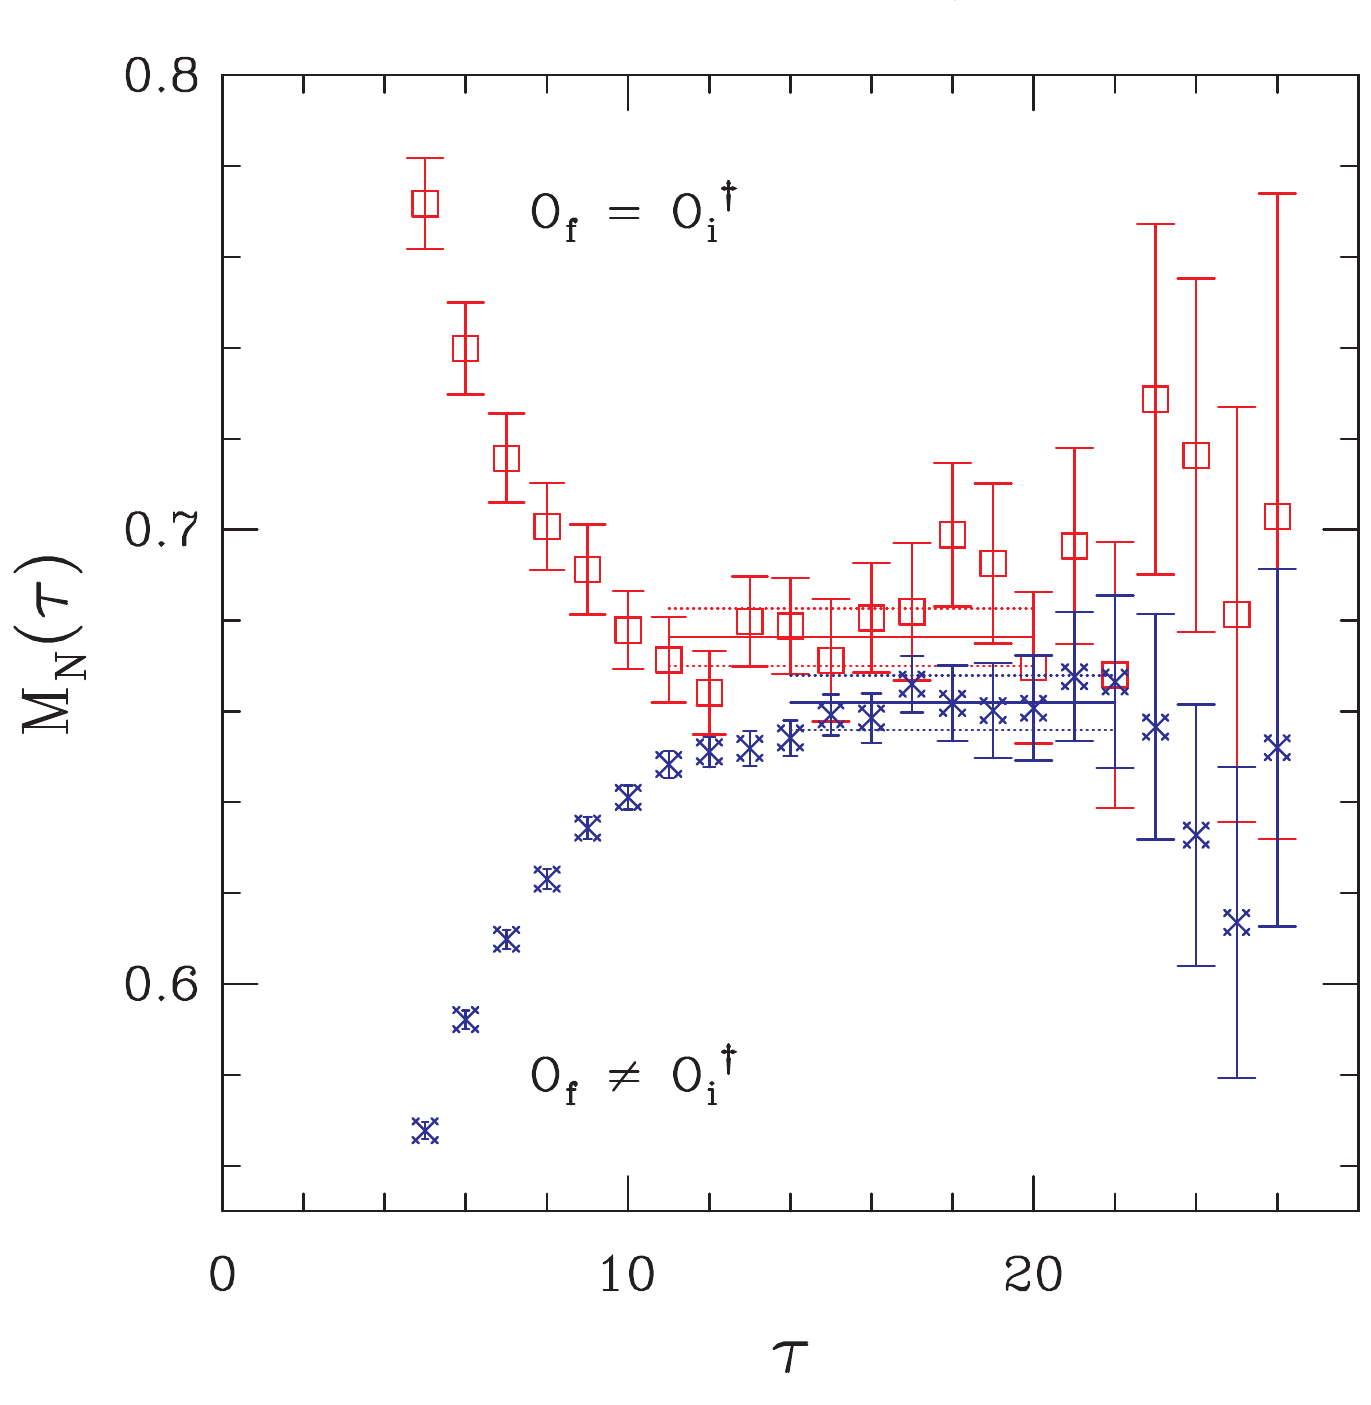
\includegraphics[width=0.8\textwidth]{images/fig23.png}
\caption{$M_N$ 随 $\tau$ 变化的有效质量图。其余与图~\ref{fig:22} 相同。}
\label{fig:23}
\end{figure}

\begin{itemize}
\item 统计误差随 $\tau$ 增大而增长，$\pi$介子除外。其原因已由 Lepage 在 [159] 中阐明，其论证要点如下。对于具有 $N$ 条价夸克线的态，其中介子（重子）的 $N = 2(3)$，误差由关联函数的平方控制，该平方含有 $2N$ 条线。因此，平方关联函数中能量最低的态，对介子是双$\pi$态，对重子是三$\pi$态。于是，当信号按 $\exp(-M \tau)$ 衰减时，噪声仅按 $\exp(-M_\pi \tau \times N/2)$ 衰减。因此，对所有满足 $M > N M_\pi / 2$ 的态，误差将随 $\tau$ 增大而增大。该条件的唯一例外是$\pi$介子，其信号和噪声具有相同的 $\tau$ 依赖。
\item 在没有明显平台（信号在 $\tau$ 上延伸得不够远）的情况下，可以在式~\eqref{eq:2pt} 的求和中包含更高（径向）激发态的贡献，从而对更大的 $\tau$ 范围作拟合。这在图~\ref{fig:24} 中用一个双态拟合加以说明，该拟合涉及四个自由参数：两个振幅和两个质量。激发态的振幅和质量受到的约束较弱，因为它们试图模拟多个态的共同效果，因此此类拟合可能显著依赖于所选取的 $\tau$ 范围。可以通过迭代地改进对小 $\tau$ 处的 $\Gamma(\tau) - \Gamma_0(\tau)$ 以及对大 $\tau$ 处的基态 $\Gamma_0(\tau)$ 作单态拟合，直到覆盖整个范围，从而改进激发态参数。要增强对基态参数的置信度，更好的方法是，对用具有相同量子数的不同源算符和汇算符构造的关联函数矩阵作同时拟合。对于含有 $m$（$n$）个不同源（汇）的矩阵，同时拟合的约束更强，因为它涉及 $m + n$ 个振幅，但只有一个共同的质量。
\end{itemize}

\begin{figure}[htbp]
\centering
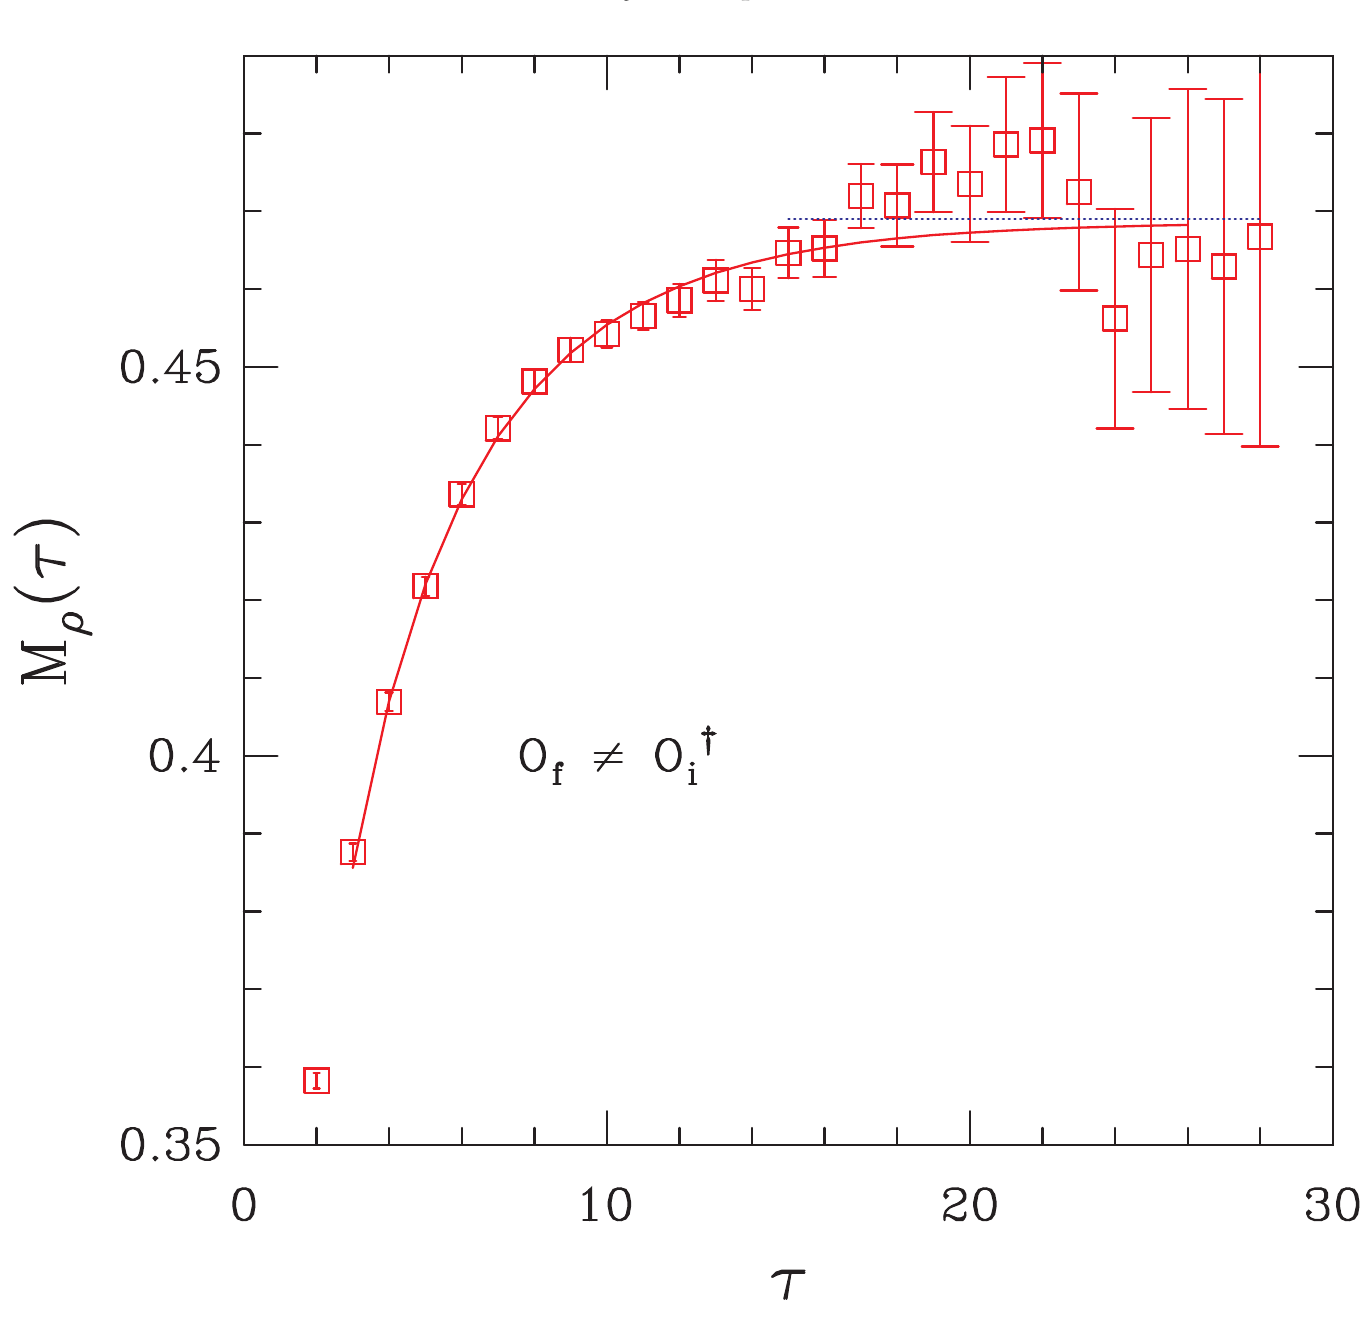
\includegraphics[width=0.8\textwidth]{images/fig24.png}
\caption{墙定域源情形下 $M_\rho$ 随 $\tau$ 变化的有效质量图。由于没有明显的平台，故对 $3 \leq \tau \leq 26$ 作包含两个态的拟合。由此类拟合得到 $\rho$ 与 $\rho^*$ 的质量。双态拟合给出的 $\rho$ 质量与对 $\tau > 15$ 数据作单态拟合得到的质量一致（蓝色点线）。}
\label{fig:24}
\end{figure}

总而言之，我们主要通过拟合 $\tau$ 的中间范围，即「平台」区域，来提取 $M$，在该区域内 $M_{eff}$ 本质上与 $\tau$ 无关。在小 $\tau$ 处激发态的影响很大，而在大 $\tau$ 处统计噪声淹没了信号。结果的精度取决于是否存在一个延伸过很大的 $\tau$ 范围、并对若干周期的相关涨落取平均的平台。图~\ref{fig:22}、\ref{fig:23} 和图~\ref{fig:24} 中的数据表明，对于在 $1/a = 2.3$ GeV 处、大小为 $32^3 \times 64$ 的 170 个格点，这一点对$\pi$介子成立，但对矢量介子和重子等其他态则仅是勉强成立。我们目前的估计是，大约需要 1000 个独立的格点才能获得可靠的信号，从而在夸克质量分别处于 $m_s - m_s/4$ 范围内时使重子质量达到 0.1--0.4\% 的精度。

假设上述步骤已经完成，并且我们对作为夸克质量、$a$、$L$ 以及动力学费米子味道数 $n_f$ 之函数的强子质量有了可靠的估计，那么最终我们就有条件将它们与实验数据进行比较。

\section{轻介子与重子谱的现状}

对QCD的第一个检验是用四个输入参数 $m_u$、$m_d$、$m_s$ 和 $\alpha_s$ 的模拟来重现赝标介子（PS = $\{\pi, K, \eta\}$）、矢量介子（V = $\{\rho, K^*, \omega, \phi\}$）、八重态重子（$B_8 = \{N, \Sigma, \Xi, \Lambda\}$）和十重态重子（$B_{10} = \{\Delta, \Sigma^*, \Xi^*, \Omega\}$）的质量。我将假设格点足够大，有限尺寸效应可以忽略。其余重要问题有
\begin{itemize}
\item 模拟主要是在淬火近似下进行的。这些计算与其说是检验QCD，不如说是量化QQCD的精度。
\item 同位旋破缺效应和电磁贡献被忽略。
\item 模拟是在非物理的夸克质量值下进行的，典型范围是 $[2m_s - m_s/4]$。为得到物理结果，需利用（淬火）手征微扰论所预言的函数形式将数据外推到 $m = (m_u + m_d)/2$。
\end{itemize}

分析的第一步是将数据外推到 $m$ 和 $m_s$ 的物理值。最简单的 Ans\"atze 是最低阶手征表达式
\begin{equation}
\begin{aligned}
M_{PS}^2 a^2 &= B_{PS} a^2 (m_1 + m_2)/2 + \cdots, \\
M_V a &= A_V + B_V a (m_1 + m_2)/2 + \cdots, \\
M_\Sigma a &= A_N + 4F m a + 2(F - D) m_s a + \cdots, \\
M_\Lambda a &= A_N + 4(F - D/3) m a + 2(F + D/3) m_s a + \cdots, \\
M_{10} a &= A_{10} + B_{10} a (m_1 + m_2 + m_3)/3 + \cdots.
\end{aligned}
\label{eq:chiral}
\end{equation}

由这些拟合我们确定常数 $A_V$、$A_N$、$A_{10}$ 以及 $B_{PS}$、$B_V$、$F$、$D$、$B_{10}$。然后利用适当的一组，例如 $A_V$、$B_{PS}$、$B_V$ 或 $A_{10}$、$B_{PS}$、$B_{10}$，来固定三个输入参数 $1/a$、$m$、$m_s$。除非另有说明，下面的讨论将假定 $m$、$a$ 和 $m_s$ 已分别用 $M_\pi$、$M_\rho$ 和 $M_\phi$（或等价地 $M_{K^*}$）确定。接下来的问题便是——其余态的质量与实验数值比较得如何？

这种检验QCD（或量化淬火近似）的简单分析可能在两方面有所欠缺。第一，数据可能显著偏离线性关系式~\eqref{eq:chiral}。在这种情况下，由于自由参数数目的增加，分析会变得复杂得多；可能的领头非线性项包括 $O(m^2)$ 修正和手征对数。要将它们分辨开来，需要 $m_s/4 - 3m_s$ 范围内多个 $m_q$ 取值处的非常精确的数据；然而，这种出现比「朴素」夸克模型所预言更丰富物理的可能性令人兴奋。第二个可能的不足是，用来固定 $a$、$m$、$m_s$ 的不同态组给出不同的结果。这一失败可能有三方面原因：(i) 在显著更重的 $m_q$ 值下由模拟提取的系数会随夸克质量的减小而变化；(ii) 这些差异是离散化误差的假象，在 $a = 0$ 极限下消失；(3) 淬火误差。当前数据显示出对 $m_q$ 的拟合中存在非线性项的迹象 [156,160]。此外，由不同组提取的 $a$、$m$、$m_s$ 显著不同，上述三方面原因都有贡献。因此，当前分析的重点是首先分辨并量化各种假象的贡献。下面我将简要说明这些效应。

让我从手征拟合中非线性项存在的证据开始。图~\ref{fig:25} 是矢量介子质量随夸克质量变化的示例 [156]。该图清楚地表明，为了量化这些偏差，需要在大的 $m_q$ 范围内有非常精确的数据。在 $\sim 0.5\%$ 的统计精度下，线性拟合在 $0.02 \leq ma \leq 0.04$（对应 $50 \leq m \leq 100$ MeV）范围内可行，但对整个范围则不行。领先的手征修正正比于来自手征圈图的 $m^{3/2}$，以及 $m^2$。包含其中任一项都可以对整个范围作拟合，而数据还不够精确，无法将它们区分开来。这些非线性项的影响似乎很小，例如在拟合中包含任一高阶项之后，外推到 $m$ 处 $M_\rho$ 的变化约为 $< 1\%$。

\begin{figure}[htbp]
\centering
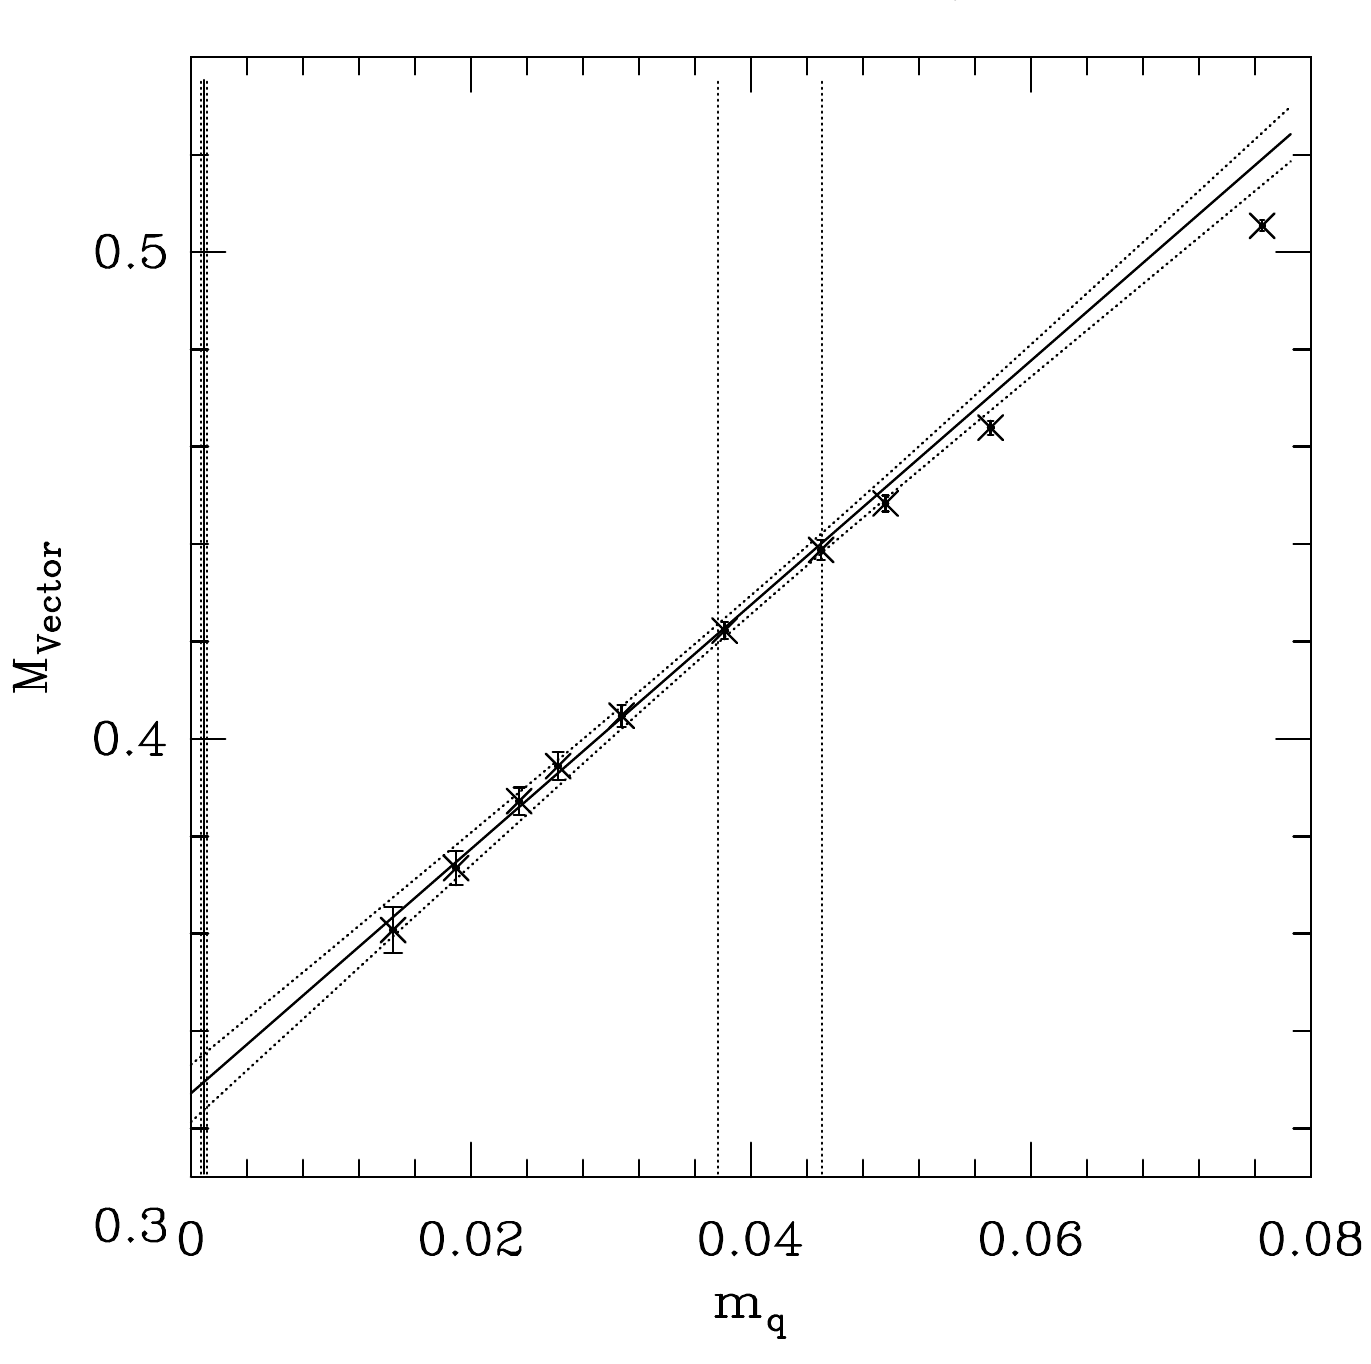
\includegraphics[width=0.8\textwidth]{images/fig25.png}
\caption{$M_{vector}$ 随夸克质量 $m$ 变化的图。数据引自 [156]，是在 $\beta \equiv 6/g^2 = 6$、对应 $1/a = 2.33(4)$ GeV 的 $32^3 \times 64$ 淬火格点上得到的。线性拟合针对最轻的六个点。竖线表示 $m$ 以及 $m_s$ 的估计范围。}
\label{fig:25}
\end{figure}

对淬火近似的第一个检验是它能否重现介子扇区的超精细劈裂。图~\ref{fig:26} 显示了一些当前的数据。唯一的输入量是标度 $1/a$，它用于将格点质量换算为物理单位。如果用 $M_\pi$ 和 $M_\rho$ 分别设定 $m$ 和 $1/a$，那么各曲线按其构造必然要穿过 $M_{PS} = M_\pi$ 处的实验点。对定标量作不同的选择会改变 $1/a$，并整体平移各曲线。

\begin{figure}[htbp]
\centering
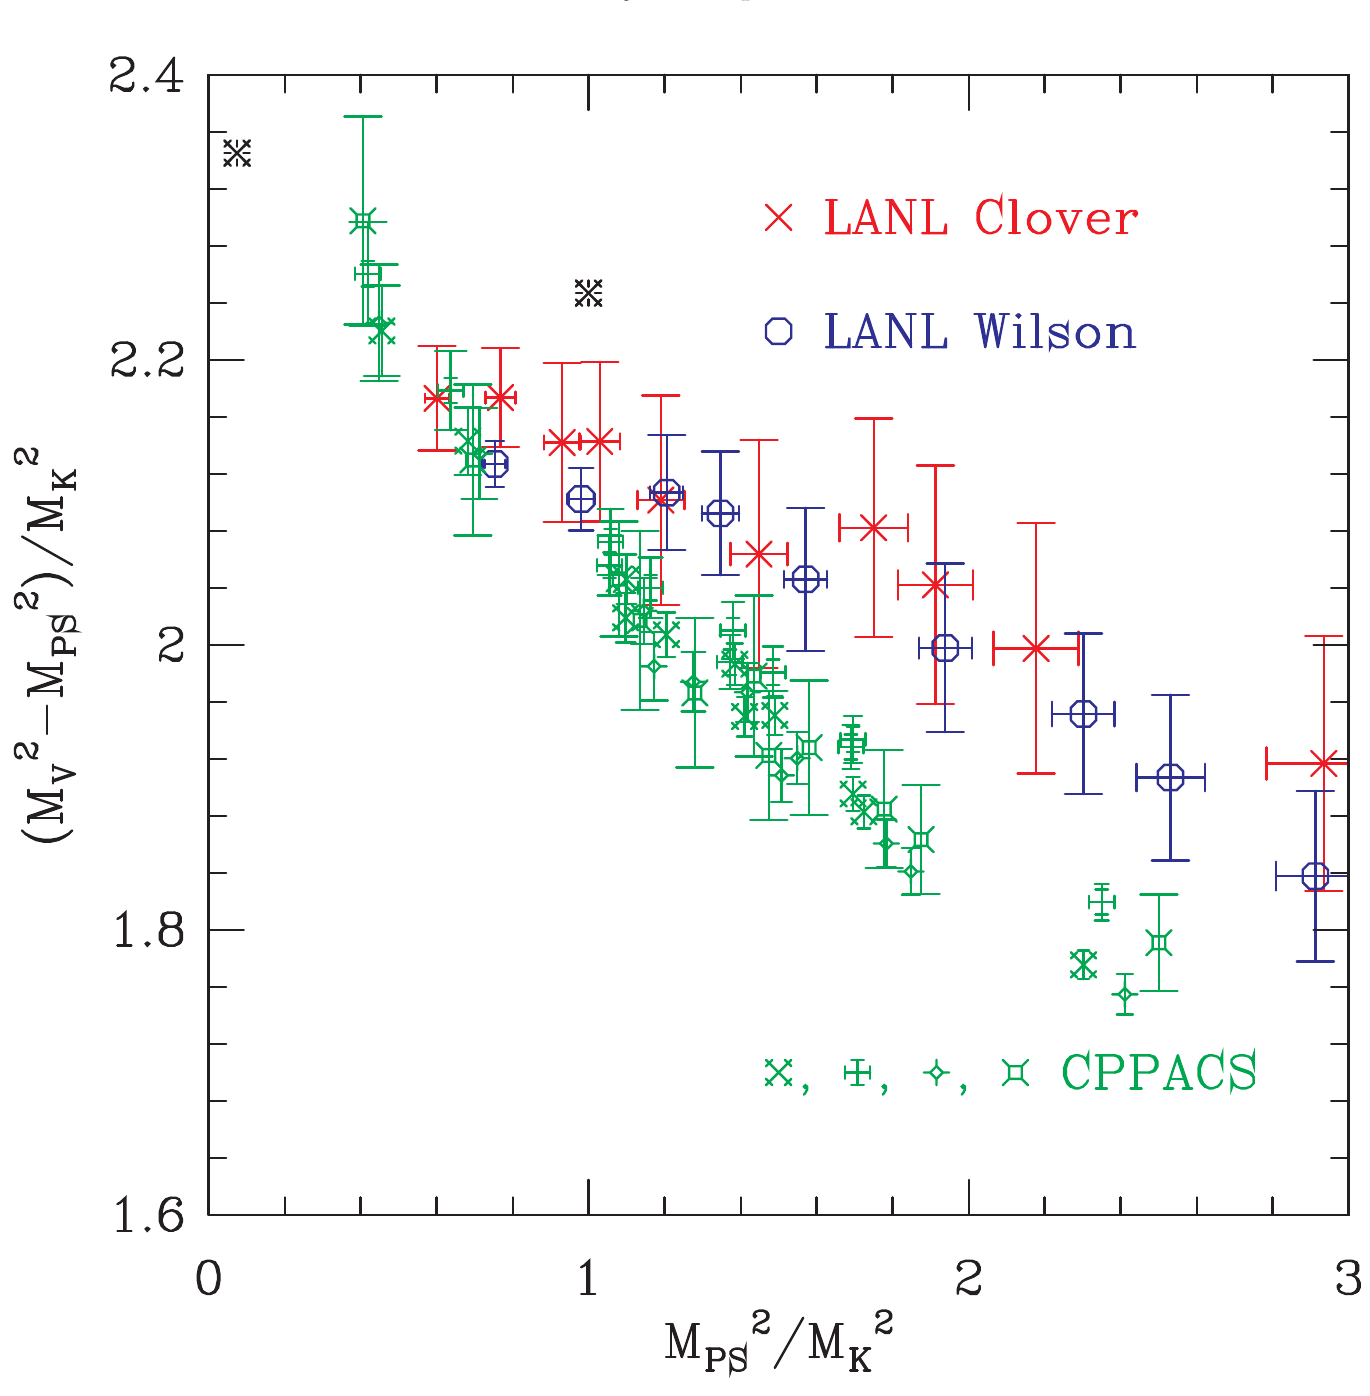
\includegraphics[width=0.8\textwidth]{images/fig26.png}
\caption{介子扇区的超精细劈裂。淬火数据来自 (i) 采用威尔逊费米子的 LANL 合作组（蓝色八边形）[156]，(ii) 采用蝌蚪图改进三叶草费米子的 LANL 合作组（红色叉号）[162]，以及 (iii) 在 $\beta = 5.9, 6.1, 6.25, 6.47$ 处采用威尔逊费米子运行的 CP-PACS 合作组（绿色异形叉号、加号、菱形和方块）[161]。实验点用爆炸形符号显示。}
\label{fig:26}
\end{figure}

另一方面，任意给定点处的斜率与格点标度无关，因此是更稳健的格点预言。出于这一原因，量 $J \equiv M_V \, \partial M_V / \partial M_{PS}^2$ 常被用作对超精细劈裂的检验。格点数据（综述见 [161]）给出的 $J$ 值约小 $\sim 20\%$。这一差异的另一个表现将出现在第~20 节中，我将说明用 $M_K$ 与用 $M_{K^*}$（或 $M_\phi$）固定的 $m_s$ 估计相差约 $\sim 15\%$。

图~\ref{fig:26} 所示数据允许两种比较。首先，八边形（蓝点）和叉号（红色）是 LANL 用威尔逊和蝌蚪图改进三叶草 Dirac 作用量在同一批 170 个 $\beta = 6.0$ 淬火 $32^3 \times 64$ 格点上的数据 [156,162]。并没有发现三叶草费米子带来任何显著改进。其次，异形叉号、加号、菱形和方块（绿点）是 CP-PACS 合作组在 $\beta = 5.9, 6.1, 6.25, 6.47$ 处用威尔逊费米子得到的数据 [161]。四个 $\beta$ 值处的数据是一致的。这两种比较都表明，较小的劈裂并非由离散化误差造成。

图~\ref{fig:26} 中的数据还显示，在重于 $m_s$ 的夸克质量处，CP-PACS 与 LANL 的威尔逊费米子结果之间存在差异。这令人惊讶，因为在该区域两个合作组对矢量介子和赝标介子质量都有可靠的测量。罪魁祸首是格点标度。结果表明，由 LANL 数据估计的 $1/a$ 比通过对 CP-PACS 数据插值得到的值大 3\%。调整 LANL 的标度会整体平移其数据，使所有结果相互重叠。

由这一数据及其他的淬火数据得出的结论是，劈裂的结果偏小。尽管在我看来，离散化误差的大小尚未完全厘清，但这些偏差被认为主要源于淬火近似的使用。

关于采用威尔逊作用量的重子八重态和十重态质量劈裂的最全面讨论见 [156]。注意，由于该计算只在一个 $1/a \approx 2.3$ GeV 处进行，因此离散化误差并未被分辨。有两个重要观测。(i) 重子八重态的质量劈裂表现出显著的非线性，例如 $M_\Sigma - M_\Lambda$ 对夸克质量的依赖如图~\ref{fig:27} 所示。

\begin{figure}[htbp]
\centering
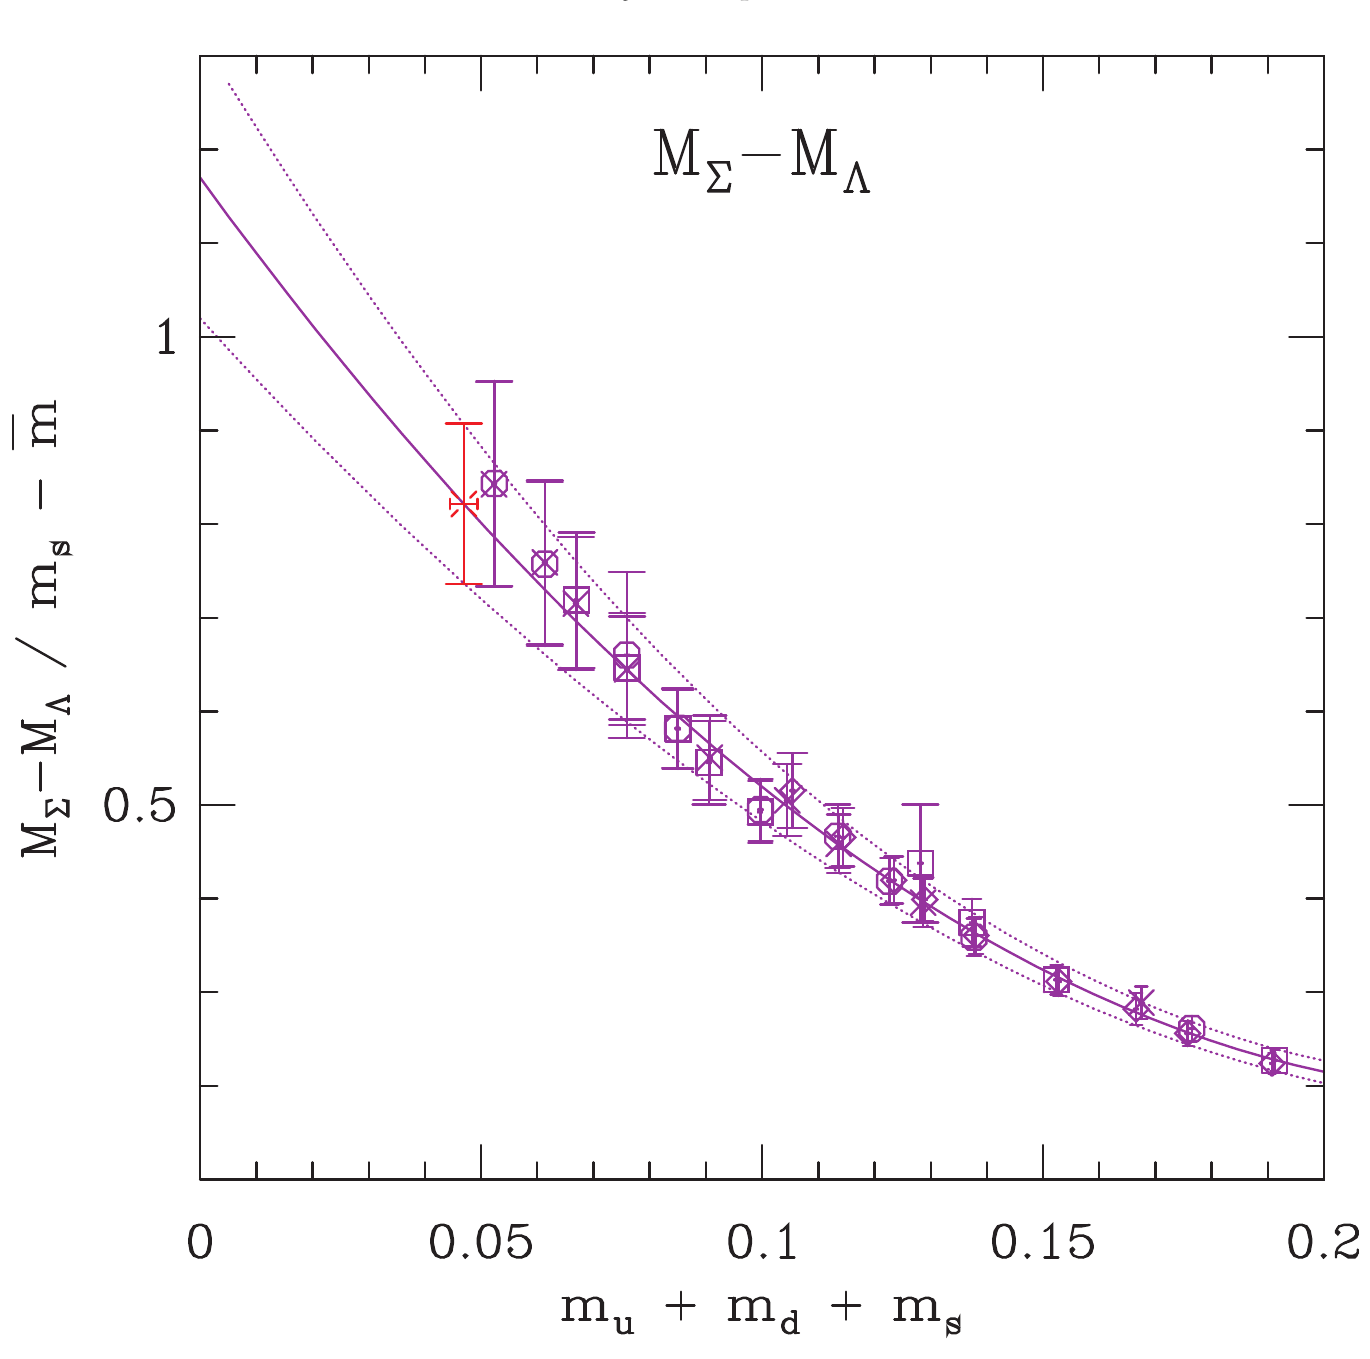
\includegraphics[width=0.8\textwidth]{images/fig27.png}
\caption{对 $(M_\Sigma - M_\Lambda)/(m - m_s)$ 的二次拟合，其中包括由完全非简并夸克组成的重子 [156]。外推到物理点的值用最左侧的爆炸形符号显示。式~\eqref{eq:chiral} 所示的线性关系本会预言一个常数值。}
\label{fig:27}
\end{figure}

非线性项显著增大了劈裂，且外推到 $m$ 得到的结果与实验值大致一致。(ii) 十重态重子质量表现出对 $m_1 + m_2 + m_3$ 的线性行为，并且无论选择 $m_s(M_K)$ 还是 $m_s(M_\phi)$，劈裂的结果都偏小。

最先进的威尔逊费米子数据由 CP-PACS 合作组获得。数据已在四个格距值处取得，因此可以对 $a = 0$ 作可靠的外推。遗憾的是，数据尤其是重子质量劈裂尚未被充分分析，因此这里给出的一些观测应被视为初步结果。图~\ref{fig:28} 取自 Yoshie 在 LATTICE 97 上的综述 [161]，是 CP-PACS 的手征拟合版本。

\begin{figure}[htbp]
\centering
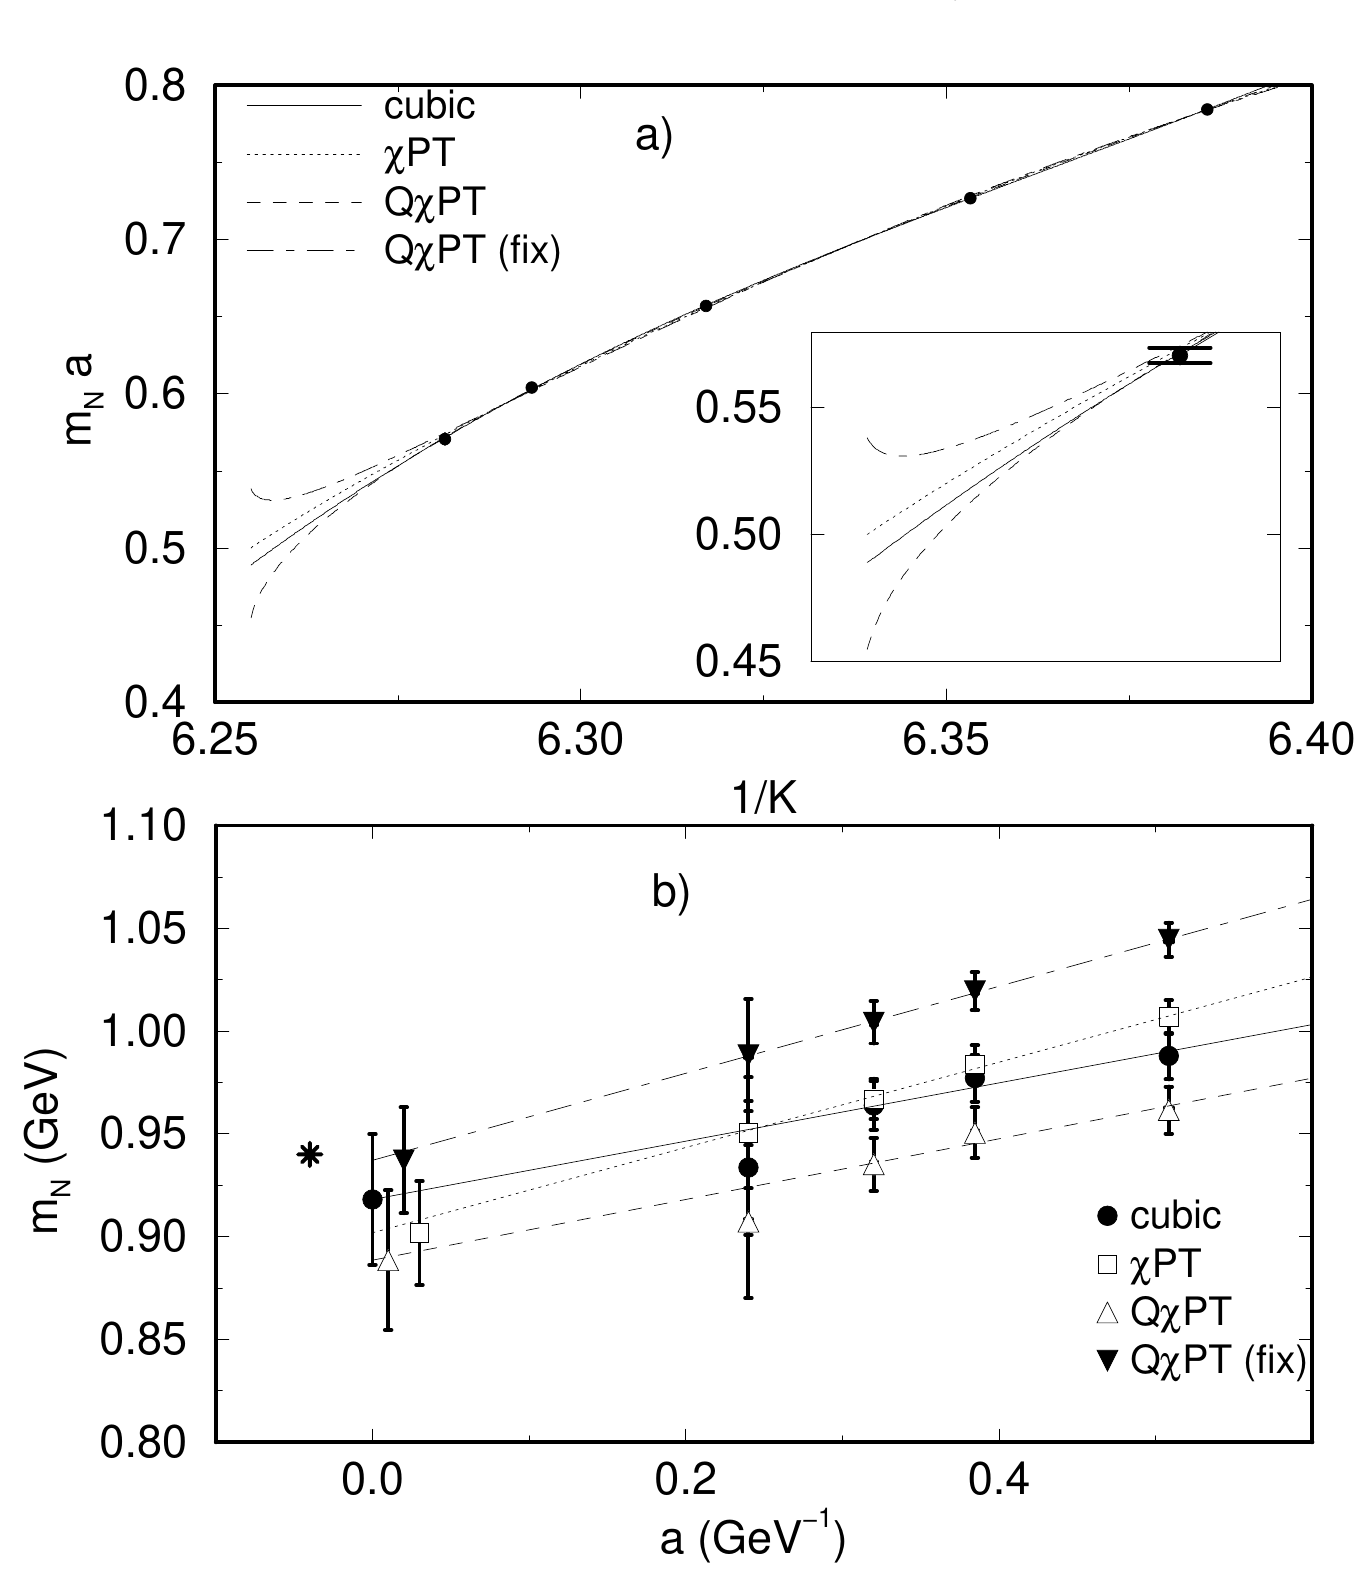
\includegraphics[width=0.8\textwidth]{images/fig28.png}
\caption{(A) CP-PACS 合作组采用威尔逊规范作用量和费米子作用量对 $M_{nucleon}$ 数据的手征拟合。数据表现出负曲率，不过需要更多的点才能区分三次拟合 $M_N = c_0 + c_1 M_\pi + c_2 M_\pi^2 + c_3 M_\pi^3$ 与 $\chi$PT（$c_1 = 0$）、Q$\chi$PT（$c_3 = 0$）、$\chi$PT（固定）（$c_1 = -0.53$）等拟合。(B) 用 (A) 中不同手征表达式得到的核子质量的连续外推。图引自 [161]。}
\label{fig:28}
\end{figure}

他们发现，在 $m_s/4 - m_s$ 范围内，只有核子和 $\Lambda$ 粒子表现出任何显著的曲率。尽管需要更多夸克质量值处的数据来分辨领头高阶修正的形式，他们分析的结论是：在核子数据拟合中发现的负曲率大到足以将淬火估计的 $M_N / M_\rho$ 改变为与实验值 $\sim 1.22$ 几乎完美一致。（这种负曲率在 1997 年以前报道的计算中并未被看到/分辨出来，因此通常报道的是 $1.3 - 1.4$ 范围内更高的值。）他们对不同手征拟合结果向 $a = 0$ 的外推如图~\ref{fig:29} 所示。

\begin{figure}[htbp]
\centering
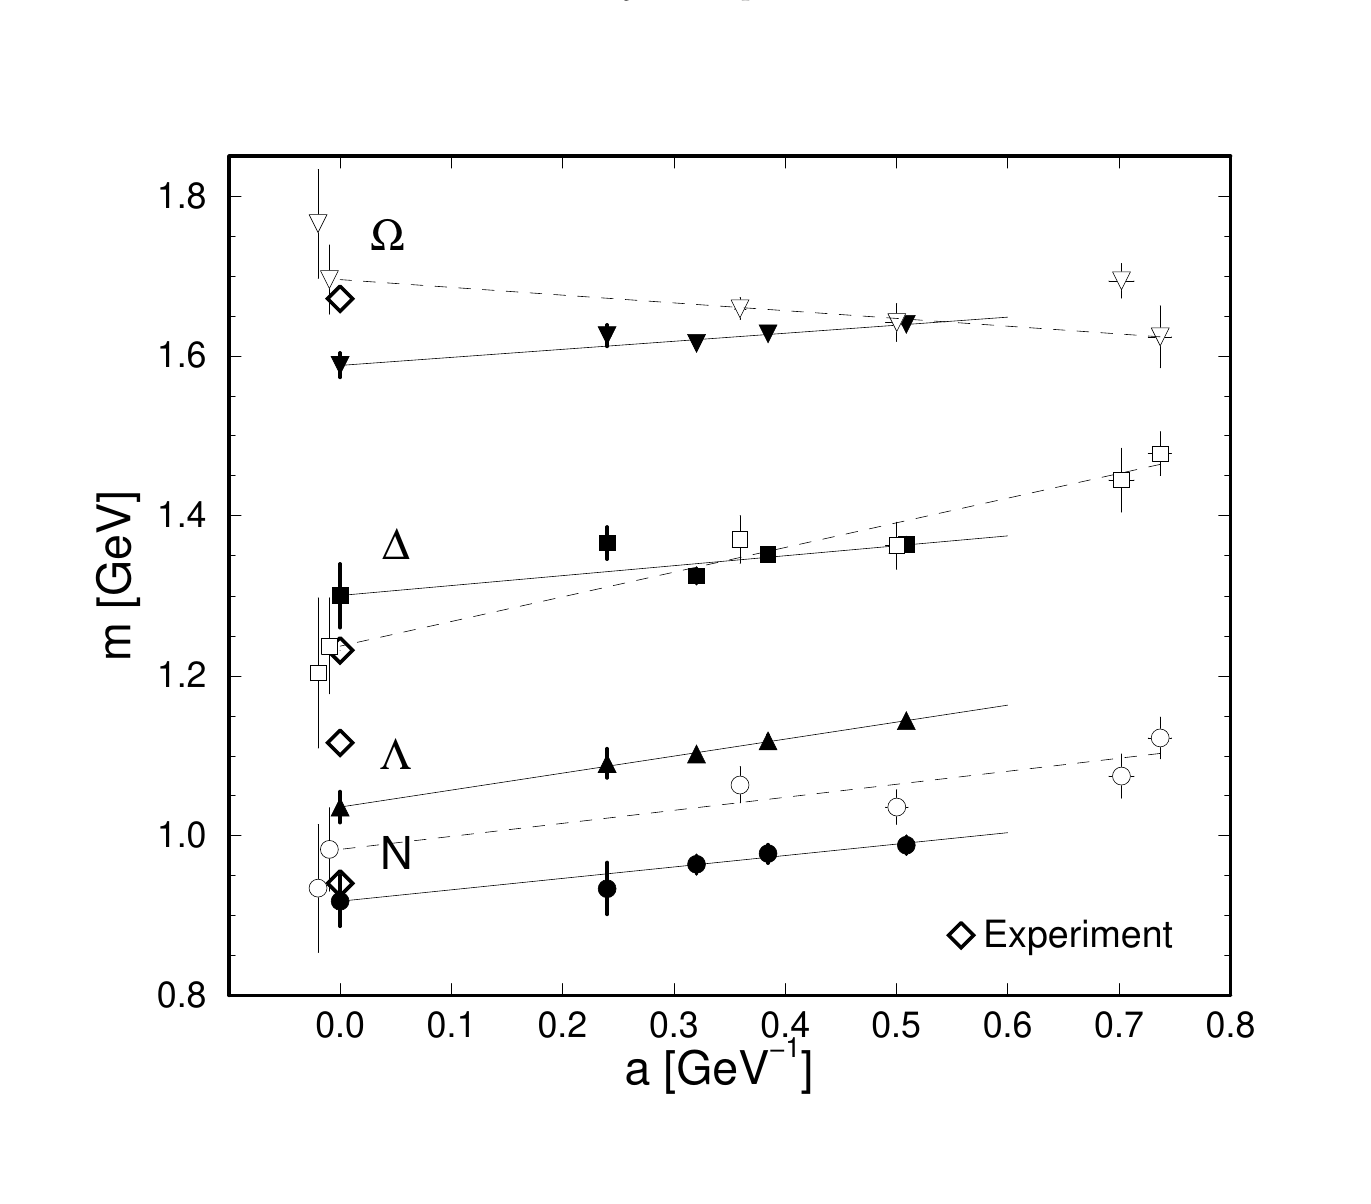
\includegraphics[width=0.8\textwidth]{images/fig29.png}
\caption{CP-PACS 合作组得到的核子、$\Lambda$、$\Delta$ 和 $\Omega$ 质量的连续外推。标度 $a$ 由 $M_\rho$ 设定。同时显示了 GF11 合作组此前最好的结果（空心符号）。实验值用菱形符号显示。图引自 [161]。}
\label{fig:29}
\end{figure}

其次，他们确认十重态质量对夸克质量是线性的，且即使在向 $a = 0$ 外推之后，无论用 $m_s(M_K)$ 还是 $m_s(M_\phi)$，劈裂的结果都偏小。他们对重子八重态劈裂的完整分析将很快发表。

图~\ref{fig:30} 给出了取自 [161]、采用威尔逊作用量的淬火结果的最终总结。

\begin{figure}[htbp]
\centering
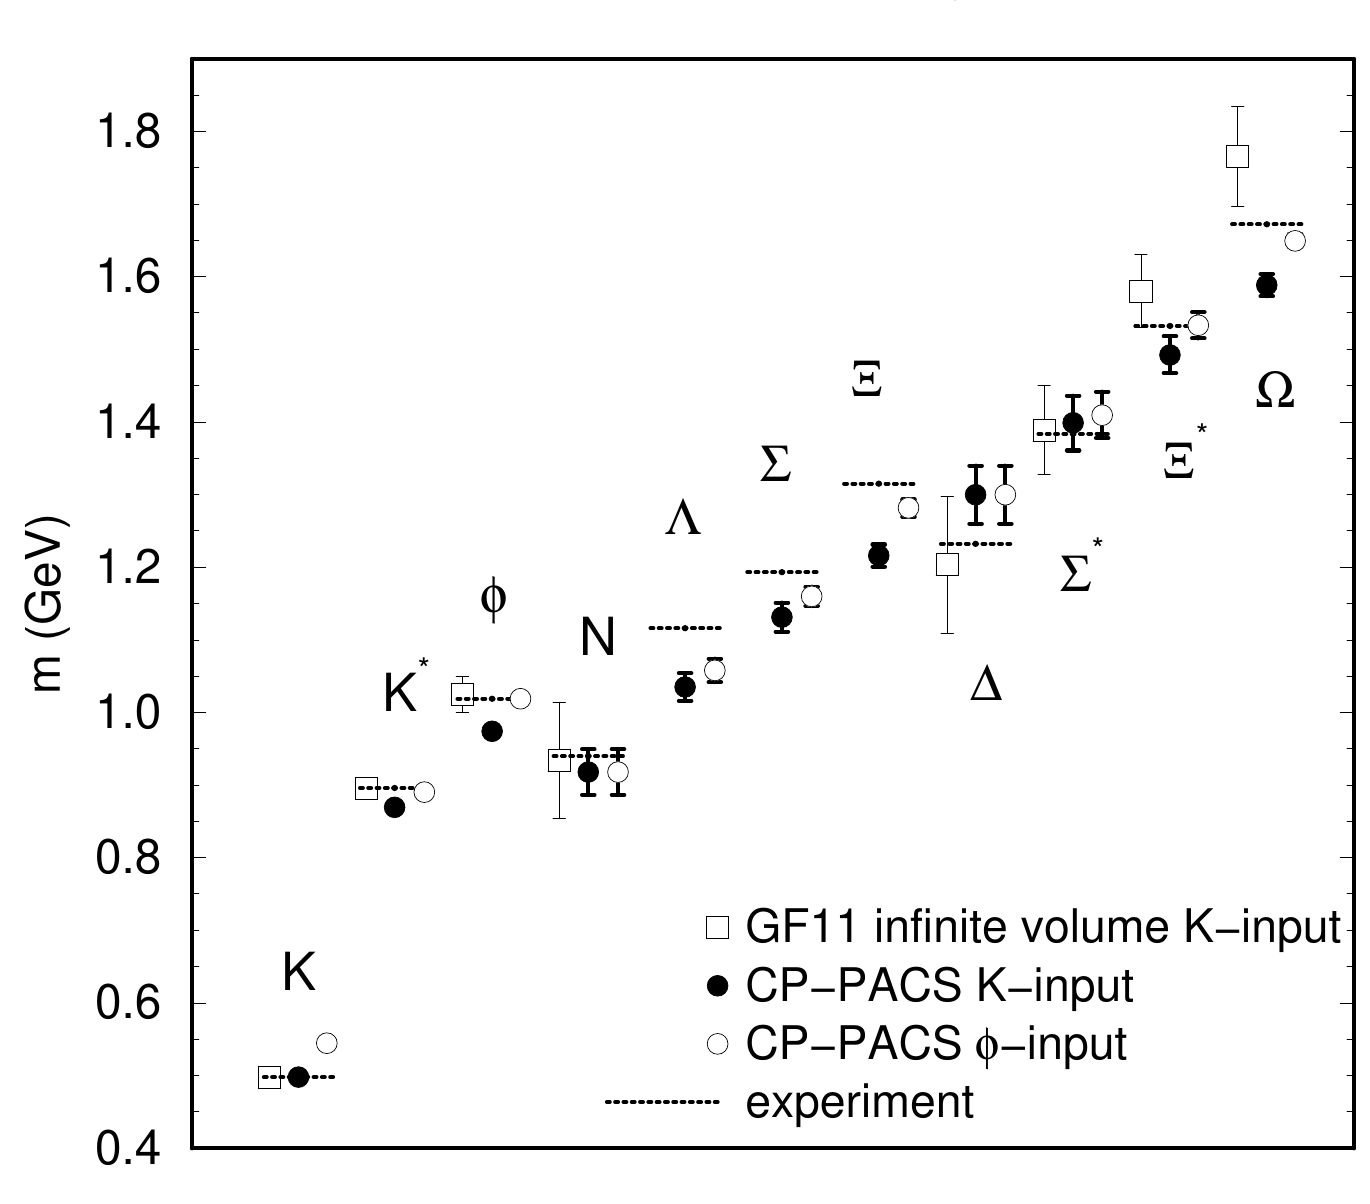
\includegraphics[width=0.8\textwidth]{images/fig30.png}
\caption{CP-PACS 合作组在 $a = 0$ 外推之后并采用威尔逊费米子得到的介子和重子质量的最先进结果。标度 $a$ 用 $M_\rho$ 设定，$m$ 用 $M_\pi$ 设定。对设定 $m_s$ 的两种方式——$M_K$ 和 $M_\phi$——给出了结果，并且很明显两者都不能给出重子八重态和十重态中正确的劈裂。数据引自 [161]。}
\label{fig:30}
\end{figure}

该图将近期 CP-PACS 外推到 $a = 0$ 的结果与 GF11 合作组此前最好的计算作了比较。从这幅图中应学到的主要教训是，似乎并不存在一个奇异夸克质量值，能够使所有介子和重子态同时匹配。在讨论夸克质量提取时我将回到这一点。显而易见的问题是——这一偏差是否是淬火近似的假象？我的看法是，我们目前还不能完全掌控淬火数据，因此不能把淬火指认为唯一的罪魁祸首。例如，$m_q$ 本身的定义就有 $O(m_q a)$ 阶的修正，将其纳入会改变手征拟合的性质。要充分理解离散化误差，我们需要等待交错费米子和 $O(a)$ 改进三叶草公式下同样高质量的数据，然后再宣称确定性的淬火数值。

截至撰写本文时，动力学模拟已真正开始，但尚缺乏在多个 $a$ 值、采用不同作用量的精确定量结果。因此，我认为现在从中得出任何结论还为时过早。关于 $n_f = 2$ 结果的最新状况报告，参见 Yoshie 和 Gottlieb 近期的综述 [161,160]。

\section{衰变常数}

除了从两点关联函数的指数衰减速率提取质量之外，振幅 $\langle n | O | 0 \rangle$ 还给出衰变常数。例如，轴矢流矩阵元 $\langle \pi | A_\mu(x) | 0 \rangle = i f_\pi p_\mu \exp(i p \cdot x)$ 给出$\pi$介子衰变常数。近期衰变常数的一些结果已由 Martinelli 教授在本学校讲习班上作过综述，其他近期综述可见 [163,164]。我这里想解释的技术要点是，为什么衰变常数的误差远大于质量的确定中的误差。首先，由式~\eqref{eq:2pt} 注意到，对于质量确定中的 1\% 误差，衰变振幅的分数误差约为 $\approx \exp(0.01 m \tau) - 1 \approx 0.005 m \tau$。由于对于 $1/a \sim 2$ GeV 的格点，拟合中通常有 $m\tau \approx 5$，衰变常数的误差约为 $\sim > 3\%$。其次，对于任何给定的组态，关联函数在 $\tau$ 上是高度相关的。对每个单独组态绘制 $\log(\Gamma(\tau))$，会注意到主要的涨落出现在整体归一化中，即振幅。这些涨落随 $m_q$ 减小而极快地增长，实际上正是第~10 节所讨论的异常组态的信号。这两类误差来源合在一起，使衰变常数的统计误差远大于 $M_{eff}$ 的提取中的误差。此外还必须加上来自定域流重整化常数的系统不确定性。

\section{胶球谱的格点计算}

胶球（主要由胶子组成的强子态）的存在是QCD一个重大的未经检验的预言。假定QCD是正确理论，我们可以确定大量可能的胶球态的量子数，但还不能计算它们的质量，或它们与 $q\bar{q}$、$qq\bar{q}\bar{q}$、\ldots{} 态的混合，也无法详细了解其产生和衰变机制。各种模型如袋模型、磁通管模型、求和规则等给出的质量估计彼此相差甚远，这些计算的可靠性较差。由 Burnett 和 Sharpe 汇编的理论预期总结（略为过时）可见 [165]。对胶球性质缺乏了解，对实验学家并无帮助，他们必须从 $1-2.5$ GeV 区域中不计其数的介子态里分离出这些态。显然，LQCD 计算可以通过计算谱以及它们与 $q\bar{q}$ 介子的混合发挥关键作用。

LQCD 的第一个目标是在与夸克态的混合被关掉的世界上计算淬火谱。我将只集中于 $0^{++}$ 和 $2^{++}$ 态，因为这两个态被研究得最为广泛。胶球算符 $O$ 由威尔逊圈构造。考虑位于 $xy$ 平面内的 $n \times m$ 威尔逊圈 $W^{n,m}_{xy}$。则转动不变的求和 $W^{n,m}_{xy} + W^{n,m}_{yz} + W^{n,m}_{zx}$ 投影到 $0^{++}$ 态上，而 $W^{n,m}_{xy} - W^{n,m}_{yz}$ 及其置换投影到 $2^{++}$ 态上。通过取不同尺寸圈的一个适当的线性组合，使其与物理胶球态的重叠最大化，可以改进两点关联函数中的信号。这类策略之一在 [166] 中讨论。遗憾的是，胶球关联函数中的统计信号远比介子和重子关联函数的弱。即使采用 $O(10^5)$ 个独立组态的样本，信号也延伸不过 $\tau \sim 10$ 或 $M\tau \sim 6$，在有效质量图中只是勉强有「平台」。胶球关联函数信号之所以如此之差，是因为它们测量的是与虚胶球的产生和传播相对应的真空涨落，而在介子和重子关联函数中，传播子中的夸克是作为外源加入的。

$M_{0^{++}}$ 和 $M_{2^{++}}$ 态更近期的、高统计量的结果取自文献 [166--169]。数据及其向 $a = 0$ 的外推如图~\ref{fig:31} 所示。

\begin{figure}[htbp]
\centering
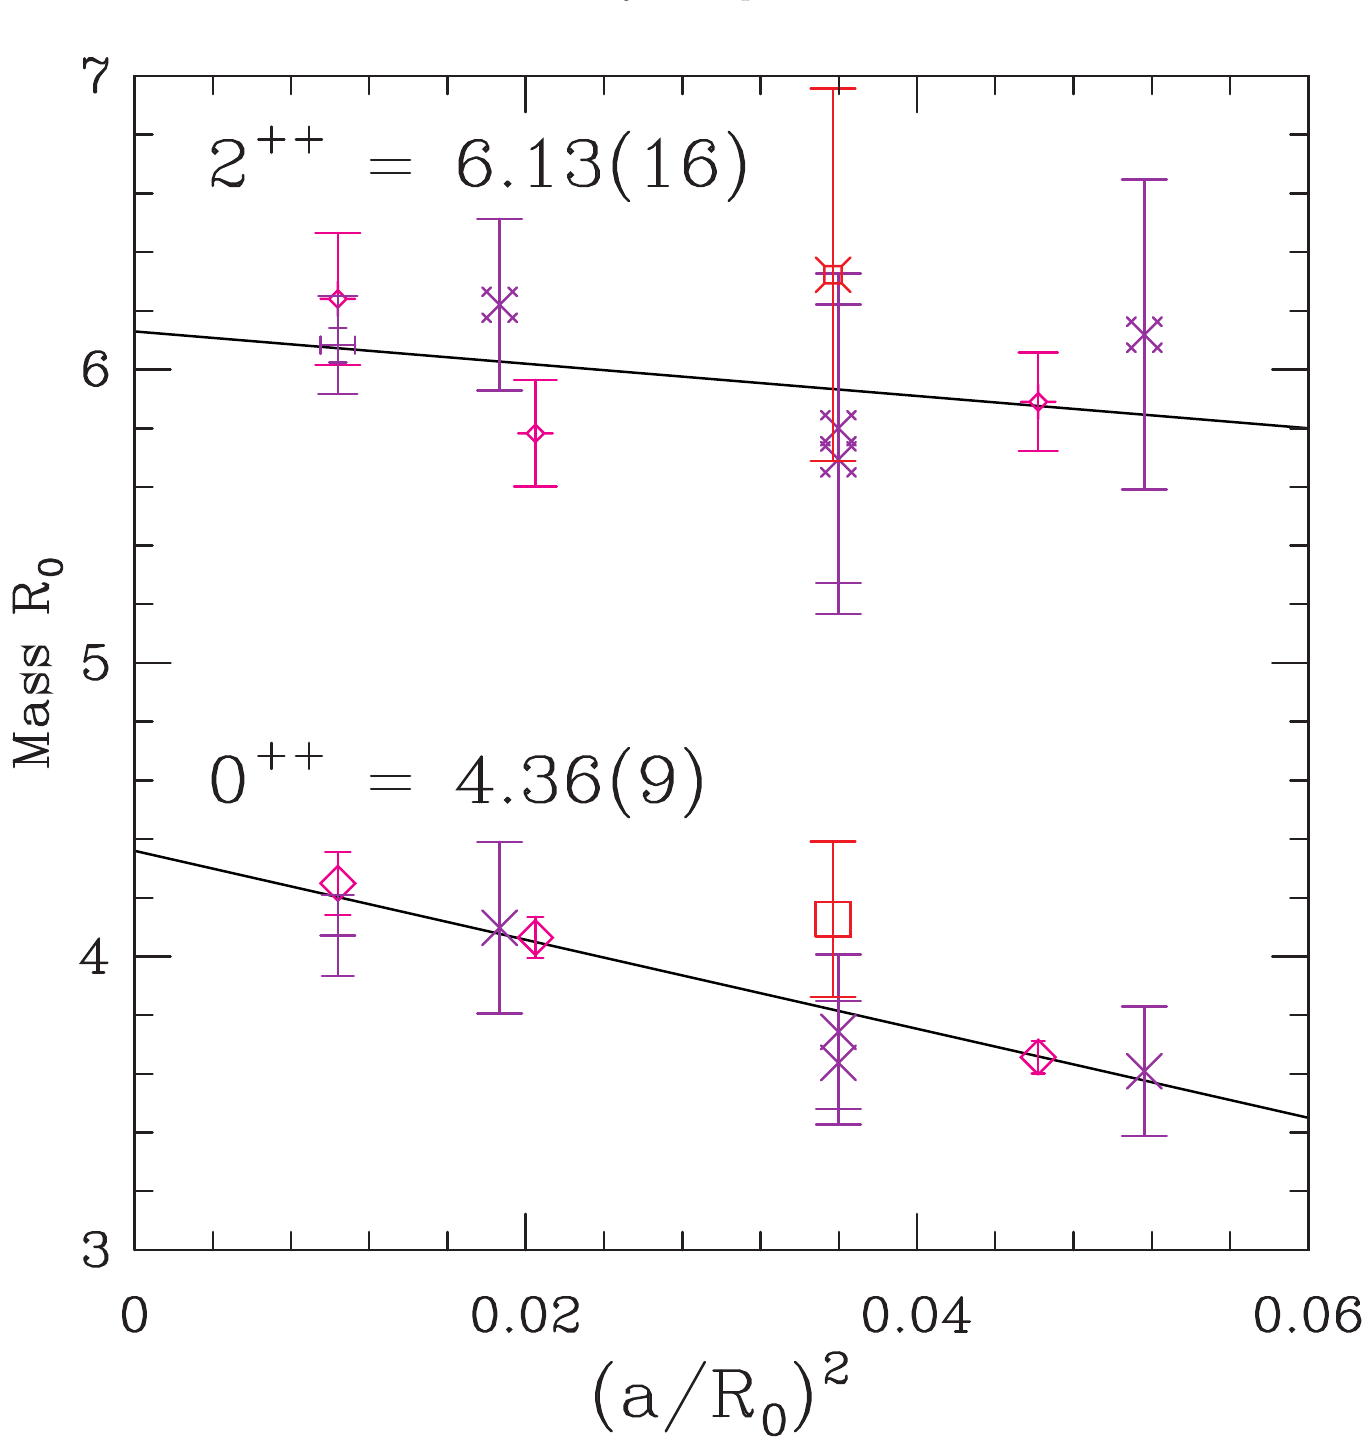
\includegraphics[width=0.8\textwidth]{images/fig31.png}
\caption{$0^{++}$ 和 $2^{++}$ 胶球质量数据向 $a = 0$ 的外推。数据来自 UKQCD-WUPPERTAL 合作组（叉号）、GF11 合作组（菱形）和洛斯阿拉莫斯（Los Alamos）合作组（方块）。格点标度用 $R_0$ 设定，它与弦张力的关系为 $1/R_0 = \sqrt{\sigma}/1.18$。}
\label{fig:31}
\end{figure}

在这幅图中，我选择用 $R_0 = 1.18/\sqrt{\sigma}$ 来设定格点标度，其中 $\sigma$ 是弦张力 [170]。该图清楚地表明，来自各合作组的格点数据完全一致，尽管 GF11 数据 [169] 的统计质量要高得多。对领头离散化误差 $a^2$ 作拟合，给出淬火理论连续极限 $M_{0^{++}} R_0 = 4.36(9)$ 和 $M_{2^{++}} R_0 = 6.13(16)$。要得到物理单位的质量，需要为 $R_0$ 或等价地 $\sigma$ 选择一个数值。这使我们回到所有淬火计算中固有的整体标度不确定性。与此分析相关的有两个问题：(i) 应当为 $\sigma$ 选择什么数值，(ii) 如果当初用 $M_\rho$ 或 $\Lambda_{QCD}$ 之类的不同量来设定标度，结果会改变多少？最常被引用的两个结果如下。UKQCD-WUPPERTAL 合作组基于选择 $\sqrt{\sigma} = 440$ MeV 而使用 $1/R_0 = 373$ MeV，得到 $M_{0^{++}} = 1626(34)$ 和 $M_{2^{++}} = 2286(60)$ MeV [170]。更新后的 GF11 合作组估计为 $M_{0^{++}} = 1648(58)$ 和 $M_{2^{++}} = 2273(116)$ MeV，使用基于 $M_\rho$ 定标的 $\Lambda^{(0)}_{QCD} = 235(6)$ MeV [171]。因此，两个组的估计是一致的，并与图~\ref{fig:31} 所示的拟合相符。所以，在我看来，基于这些拟合，当前合并的格点估计为 $M_{0^{++}} = 1640(30)(160)$ MeV 和 $M_{2^{++}} = 2280(60)(230)$ MeV，其中我额外加上了 10\% 的第二个系统误差，以计入淬火模拟固有的标度不确定性。

\section{各向异性格点上的改进作用量结果}

为缓解胶球两点关联函数信号迅速衰减的问题，Peardon 和 Morningstar 在 $a_t \ll a_s$ 的各向异性超立方格点上进行了模拟 [172]。这一技巧的优点如下。假设在各向同性格点模拟中，$M_{eff}(\tau)$ 在 $\tau = 2-4$ 之间存在一个近似平台，之后信号劣化为噪声。这样的平台很难仅从三个时间切片推断出来。另一方面，对于 $a_s/a_t = 5$ 的格点，大约有 11 个时间切片可供使用，从而大大增强了估计的置信度。使用各向异性格点确实给分析引入了一个额外参数，即 $a_s/a_t$ 或光速。他们利用在空间和时间方向上测得的势能非微扰地确定该参数。

\begin{figure}[htbp]
\centering
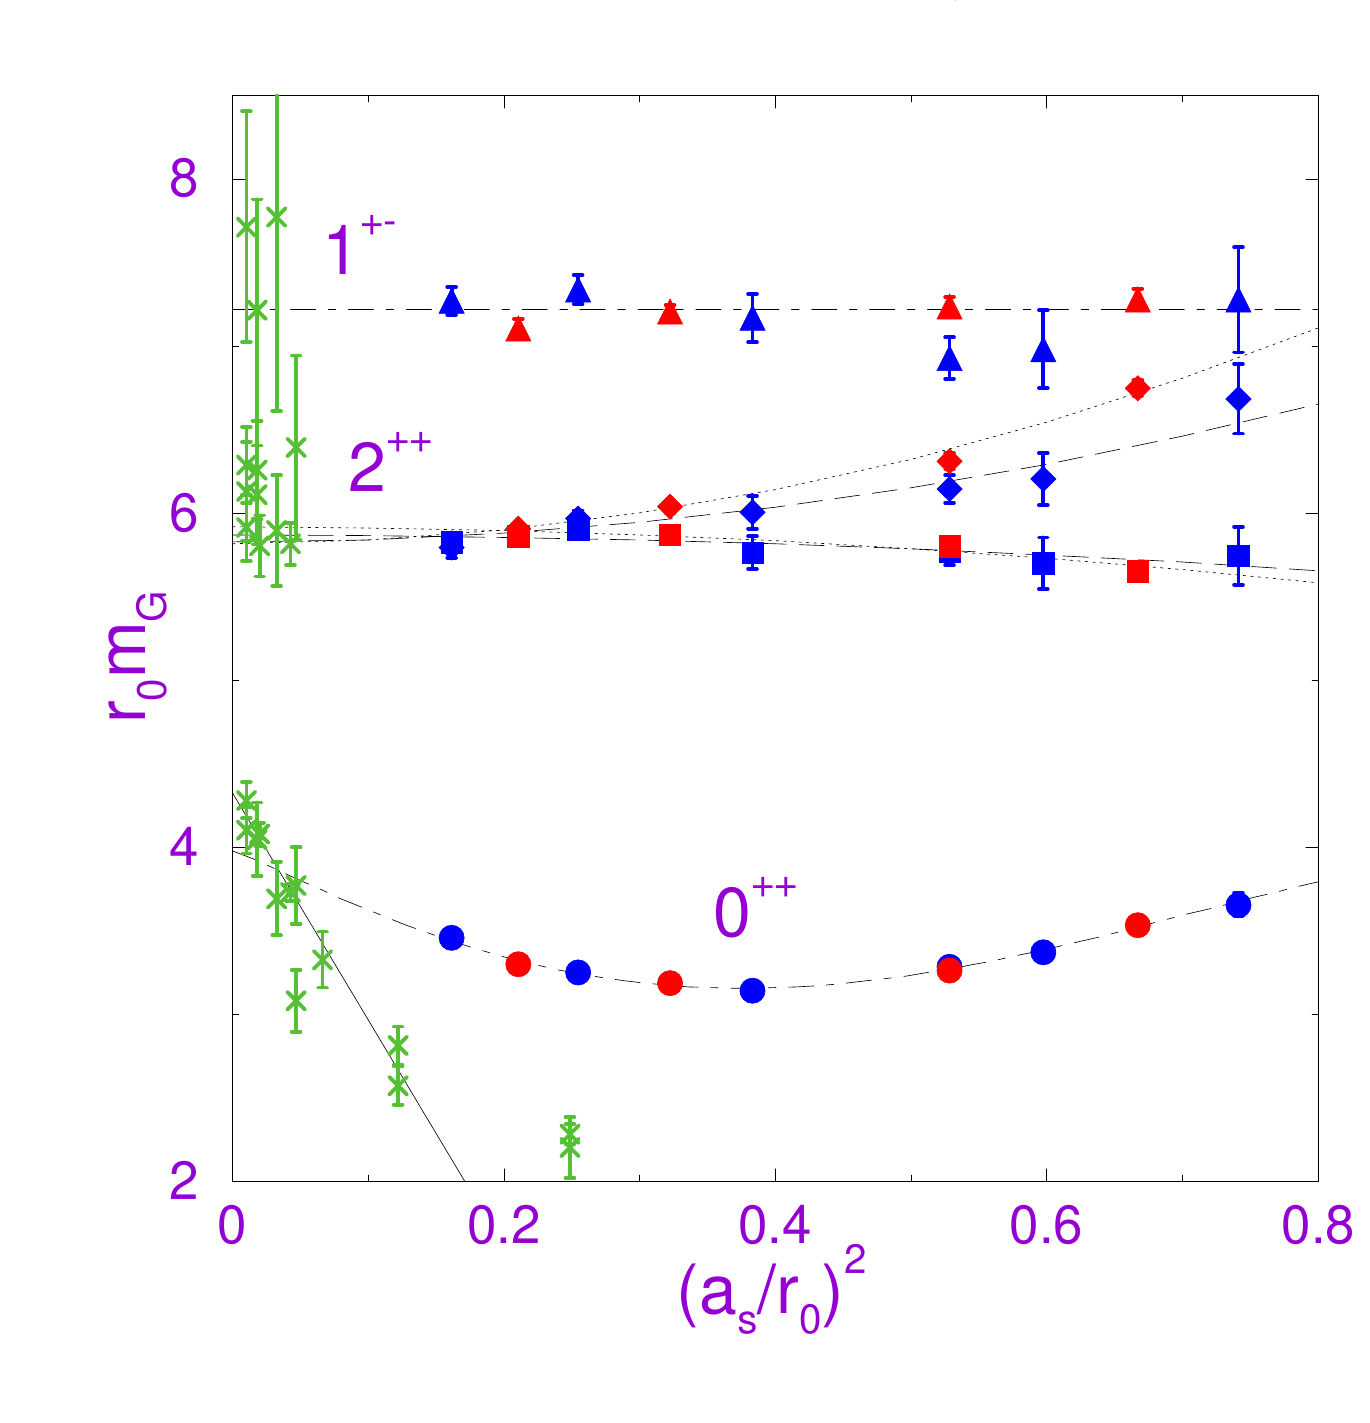
\includegraphics[width=0.8\textwidth]{images/fig32.png}
\caption{用 $R_0$ 表示的胶球质量估计随格距 $(a_s/R_0)^2$ 的变化。$\xi = 5$ 模拟中格点不可约表示 $A_1^{++}$（$0^{++}$）、$E^{++}$、$T_2^{++}$（$2^{++}$）和 $T_1^{+-}$（$1^{+-}$）的结果分别用 $\circ$、$\square$、$\star$ 和 $\triangle$（蓝色）标记。相应的红色符号表示 $\xi = 3$ 模拟的结果。取自文献 [167--169] 的威尔逊作用量模拟数据用绿色叉号显示。虚线、点线和点划线分别表示对 $\xi = 3$ 数据、$\xi = 5$ 数据以及全部数据作拟合得到的连续极限外推。实线表示威尔逊作用量数据向连续极限的外推。}
\label{fig:32}
\end{figure}

他们所做的第二项改进是调节作用量。他们将蝌蚪图改进的 L\"uscher-Weisz 胶子作用量，式~12.14，移植到各向异性格点上，并在基本耦合空间和伴随耦合空间中同时包含方格项。后者的动机是为了避免第~15 节所讨论的基本–伴随空间中的相变。

他们的新数据 [139] 证实，包含负的伴随耦合确实改善了 $M_{0^{++}}$ 的标度行为。

他们在包含负伴随耦合之前的结果如图~\ref{fig:32} 所示。改进作用量和各向异性格点的优势清晰可见。首先，计算可以在粗糙得多的格点上进行。其次，离散化误差要小得多。最后，向 $a = 0$ 外推后的数值与常规方法一致。他们的估计 $M_{0^{++}} R_0 = 3.98(15)$ 和 $M_{2^{++}} R_0 = 5.85(2)$，与其 $R_0 = 410(20)$ MeV 的估计相结合后，与上一节给出的常规模拟数值一致。因此，他们的结果为淬火估计提供了又一重确认。

让我以指向其他有趣计算的线索来结束对胶性态的讨论。其他自旋–宇称胶球态的结果可见 [168,172,173]；混合态的结果可见 [173--176]。

\section{标量夸克偶素与胶球的混合}

现象学上重要的问题是，格点估计能否帮助确定两个实验候选态 $f_0(1500)$ 或 $f_0(1710)$ 中哪一个是标量胶球。仅仅利用上述淬火估计，答案是不能。原因除了上述估计与两个候选态都重叠之外，还在于与标量夸克偶素混合的效应尚未被纳入。Lee 和 Weingarten 通过计算两点函数 $\langle S(\tau) S(0) \rangle$ 和 $\langle G(\tau) S(0) \rangle$ 开始了对混合的研究，其中 $S$ 是标量密度 $(u\bar{u} + d\bar{d})/\sqrt{2}$ 或 $s\bar{s}$，$G$ 是 $0^{++}$ 胶球算符 [171]。这些非常困难的计算的统计质量目前还不够好。因此，Lee 和 Weingarten 对角化一个近似的 $3 \times 3$ 矩阵，该矩阵主要来自现象学分析。他们随后发现，混合使 $M_{0^{++}}$ 升高约 $\sim 64$ MeV，即 $M_{0^{++}}$ 从 1640 MeV 变为 1704 MeV。此外，混合态相应的波函数解释了一些出乎意料的衰变特征，例如为什么 $f_0(1500)$ 的 $KK$ 衰变道被压低，以及为什么 $\Gamma(J/\psi \to \gamma f_0(1710)) > \Gamma(J/\psi \to \gamma f_0(1390)) \gg \Gamma(J/\psi \to \gamma f_0(1500))$。因此，Lee 和 Weingarten 预言 $f_0(1710)$ 主要是（$\sim 75\%$）一个胶球。

在得到这些预言的过程中，他们忽略了与其他（多粒子）态的混合、混合矩阵中的衰变宽度以及格点计算中的淬火误差。Lee 和 Weingarten 基于现象学论证声称，这些都是小的，不会改变他们的核心结论。希望未来的 LQCD 计算能对他们的预言提供好得多的定量验证。

\section{质量不等式}

除了给出精确数值之外，LQCD（实际上是欧几里得场论）还推动了严格质量不等式的推导。第一个这样的不等式由 Weingarten 导出，表明$\pi$介子是QCD中同位旋非零的最轻介子态 [177]。考虑介子的两点关联函数，即 $O = \bar{u}\Gamma d$，其中 $\Gamma$ 可以是 Clifford 代数的 16 个元素中的任意一个。于是
\begin{equation}
\begin{aligned}
\Gamma_{\Gamma}(\tau) &= \int d^3y\, \langle 0 | \bar{d}\Gamma u(\tau, y)\, \bar{u}\Gamma d(0, x) | 0 \rangle \\
&= \Tr\, S_F^d(0,x;\tau,y)\,\Gamma S_F^u(\tau,y;0,x)\,\Gamma \\
&= \Tr\, \Gamma\gamma_5 S_F^{d\dagger}(\tau,y;0,x)\,\gamma_5 \Gamma S_F^u(\tau,y;0,x).
\end{aligned}
\label{eq:18.4}
\end{equation}

对于$\pi$介子的特殊情况，$\Gamma\gamma_5 = 1$，因此 $\Gamma_\pi(\tau)$ 在每个组态上都取最大值。此外，当 $m_u = m_d$ 时，它是传播子模的平方。其他自旋–宇称态涉及 $\gamma$ 矩阵。由于这些矩阵既有正号也有负号，求迹中的各个旋量项会发生相消。要将关联函数的这一性质转化为关于质量的不等式，所需的第二个性质是QCD的积分测度是正的，即每个组态以相同的符号作出贡献。于是，对所有的 $\tau$ 有 $\Gamma_\pi(\tau) \ge \Gamma_\Gamma(\tau)$。由于 $\Gamma(\tau) \sim e^{-m\tau}$，该不等式意味着$\pi$介子是最轻的介子。

与此同时，Witten 和 Nussinov 导出了更多的不等式。其中的例子有
\begin{itemize}
  \item $\pi$介子中的电磁质量移动为正 [179]。具体证明的是，对任何欧几里得 $k$，有 $V_\mu^3(k)V_\mu^3(-k) - A_\mu^3(k)A_\mu^3(-k) \ge 0$。
  \item 对于价味道为 $A$ 和 $B$ 的介子，在味道单态关联函数中湮灭为胶子态的贡献可以被忽略的极限下，不等式 $2M_{AB} \ge M_{AA} + M_{BB}$ 成立 [179,178]。
\end{itemize}

最近，West 将这些方法应用/推广到胶球 [181]。他表明 $0^{++}$ 是最轻的胶球态。
